%%%% For one big one:
\documentclass[11pt]{book}
%\usepackage{amssymb}
%\usepackage{amsmath}
%\usepackage{epsfig}
%\usepackage{euscript}
%%%% For one big one:
%\documentclass[10pt,slidesonly,semrot,portrait,palatino]{seminar}
%\newpagestyle{200t}{\\Models for Binary Data \hfil}{\thepage}
%\rotateheaderstrue
%\slideframe{plain}
%\setlength{\slideframewidth}{1pt}
%\setlength{\topmargin}{0cm}
%\setlength{\oddsidemargin}{0.25in}
%\setlength{\evensidemargin}{0.25in}
\usepackage{amssymb}
\usepackage{amsmath}
\usepackage{epsfig}
\usepackage{euscript}
\newcommand{\simdot}{\stackrel{\cdot}{\sim}}
\newcommand{\bfbeta}{{\mbox{\boldmath$\beta$}}}
\newcommand{\bfep}{{\mbox{\boldmath$\epsilon$}}}
\newcommand{\bhat}{\hat{\beta}}
\newcommand{\btilde}{\tilde{\mbox{\boldmath$\beta$}}}
\newcommand{\bfmu}{{\mbox{\boldmath$\mu$}}}
\newcommand{\Var}{{\rm Var}}
\newcommand{\Cov}{{\rm Cov}}
\newcommand{\trt}{{\rm trt}}
\newcommand{\pr}{{\rm pr}}
\newcommand{\age}{{\rm age}}
\newcommand{\Sin}{\sum_{i=1}^N}
\newcommand{\Sjn}{\sum_{j=1}^N}
\newcommand{\ui}{{\bf u}_i}
\newcommand{\uj}{{\bf u}_j}
\newcommand{\bfx}{{\mbox{{\bf x}}}}
\newcommand{\bfp}{{\mbox{{\bf p}}}}
\newcommand{\hbfp}{\widehat{\mbox{{\bf p}}}}
\newcommand{\bfy}{{\mbox{{\bf y}}}}
\newcommand{\bfY}{{\mbox{{\bf Y}}}}
\newcommand{\bfZ}{{\mbox{{\bf Z}}}}
\newcommand{\bfa}{{\mbox{{\bf a}}}}
\newcommand{\bfb}{{\mbox{{\bf b}}}}
\newcommand{\bfg}{{\mbox{{\bf g}}}}
\newcommand{\bfU}{{\bf U}}
\newcommand{\bfu}{{\mbox{{\bf u}}}}
\newcommand{\bfz}{{\mbox{{\bf z}}}}
\newcommand{\logit}{{\mbox{{logit}}}}
\newcommand{\bfzero}{{\mbox{{\bf 0}}}}
\newcommand{\hbeta}{{\widehat \beta}}
\newcommand{\heta}{{\widehat \eta}}
\newcommand{\hsigma}{{\widehat \sigma}}
\newcommand{\hmu}{{\widehat \mu}}
\newcommand{\hpi}{{\widehat \pi}}
\newcommand{\cI}{{\cal I}}
\newcommand{\bsigma}{{\bar \sigma}}
\newcommand{\brho}{{\bar \rho}}
\newcommand{\bx}{ {\bar {x} } }
\newcommand{\bY}{ {\bar {Y} } }
\newcommand{\hY}{ {\widehat {Y} } }
\newcommand{\hp}{ {\widehat {p} } }
\newcommand{\hVar}{ {\widehat {Var} } }
\setlength{\topmargin}{0cm}
\setlength{\oddsidemargin}{0.25in}
\setlength{\evensidemargin}{0.25in}

%\setlength{\textheight}{21cm}
%\setlength{\textwidth}{15cm}
%\setlength{\parskip}{5mm}
%\setlength{\parindent}{0mm}
%\include{envir223}
\begin{document}
\setcounter{chapter}{6} \setcounter{page}{106}
%%%%%%%%%%%%%%%%%%%%%%%%%%%%%%%%%%%%%%%%%%%%%%%%%%%%%%%%%%%%%%%%%%%%%%%%%%%%
\chapter{Model selection in survival analysis}
Suppose we have a censored survival time that we want to model
as a function of a (possibly ) set of covariates.  Two important
questions are:
\begin{itemize}
\item  How to decide which covariates to use
\item  How to decide if the final model fits well
\end{itemize}
To address these topics, we'll consider a new example:
\\[2ex]
{\bf Survival of Atlantic Halibut - Smith et al}\\
\\[2ex]
\begin{tabular}{cccccccc}
\hline
     & {\it Surv}ival &           & {\it Tow}      & Diff & {\it Length}
& {\it Handling } & Total \\
 Obs & {\it Time} & {\it Censor}ing & {\it Dur}ation & in   &  of Fish
&  Time    & {\it log(catch)} \\
 \# & (min)  & Indicator & (min.) & {\it Depth} & (cm) &
(min.) & ln(weight) \\ \hline
 100 &  353.0 &  1  & ~30 & 15 &  39  & ~5 &  5.685 \\
 109 &  111.0 &  1  & 100 & ~5 &  44  & 29 &  8.690 \\
 113 &  ~64.0 &  0  & 100 & 10 &  53  & ~4 &  5.323 \\
 116 &  500.0 &  1  & 100 & 10 &  44  & ~4 &  5.323 \\
\vdots \\
 \hline
\end{tabular}
%%%%%%%%%%%%%%%%%%%%%%%%%%%%%%%%%%%%%%%%%%%%%%%%%%%%%%%%%%%%%%%%%%%%%%%%%%%%

\normalsize
\section{Process of Model Selection}
Collett (Section 3.6) has an excellent discussion of various
approaches for model selection.  
\newpage
\noindent 
In practice, model selection
proceeds through a combination of
\begin{itemize}
\item  knowledge of the science
\item  trial and error, common sense
\item  automatic variable selection procedures
\begin{itemize}
\item forward selection
\item backward selection
\item stepwise seletion
\end{itemize}
\end{itemize}
Many advocate the approach of first doing a univariate
analysis to ``screen'' out potentially significant variables
for consideration in the multivariate model (see Collett).
\\[2ex]
{\bf Let's start with this approach!}
\\[2ex]
\noindent
Which covariates look like they might be important?
\subsection{Automatic Variable selection procedures\\
in Stata and SAS}
\underline{\bf Statistical Software:}
\begin{itemize}
\item Stata: {\tt sw} command before {\tt cox} command
\item SAS: {\tt selection=} option on model statement of \\{\tt proc phreg}
\end{itemize}
\underline{\bf Options:}
\begin{itemize}
\item[(1)] forward
\item[(2)] backward
\item[(3)] stepwise
\item[(4)] best subset (SAS only, using {\tt score} option)
\end{itemize}
One drawback of these options is that they can only handle
variables one at a time.  When might that be a disadvantage?
\subsection{Collett's Model Selection Approach}
{See Collett, Section 3.6.1}\\[2ex]

This approach assumes that all variables are considered to be on an
equal footing, and there is no {\em a priori} reason to include any
specific variables (like treatment).
\begin{figure}[h!]
\centerline{\psfig{figure=towdur.pdf,height=1.75in} \hspace{0.25in}
\psfig{figure=length.pdf,height=1.75in}}

\centerline{\psfig{figure=depth.pdf,height=1.75in} \hspace{0.25in}
\psfig{figure=handling.pdf,height=1.75in}}

\centerline{\psfig{figure=logcatch.pdf,height=1.75in}}
\caption{Univariate KM plots of Atlantic Halibut survival
(continuous variables have been dichotomized)}
\end{figure}
\clearpage
\noindent
\underline{\bf Approach:}
\begin{itemize}
\small
\item[(1)] Fit a univariate model for each covariate, and identify the
predictors significant at some level $p_1$, say $0.20$.
\item[(2)] Fit a multivariate model with all significant univariate
predictors, and use {\em backward} selection to eliminate non-significant
variables at some level $p_2$, say 0.10.
\item[(3)] Starting with final step (2) model, consider each of
the non-significant variables from step (1) using
{\em forward} selection, with significance level $p_3$, say 0.10.
\item[(4)] Do final pruning of main-effects model (omit variables that
are non-significant, add any that are significant), using {\em stepwise}
regression with significance level $p_4$.  At this stage, you may also
consider adding interactions between any of the main effects currently
in the model, under the hierarchical principle.
\end{itemize}
Collett recommends using a likelihood ratio test for all variable
inclusion/exclusion decisions.
\\[2ex]
R fits a range of models by applying the AIC criteria described by Collett:
\begin{eqnarray*}
\mbox{minimize } ~\mbox{AIC} & = & -2 ~\log(\hat{L}) + (k*q )
\end{eqnarray*}
where $q$ is the number of unknown parameters in the model and $k$ is
typically between 2 and 6 (they suggest $k=3$).
\\[2ex]
The model is then chosen which minimizes the AIC
(similar to maximizing log-likelihood, but with a penalty for
number of variables in the model)
\\[2ex]
\underline{\bf R command for forward Selection}\\[2ex]
We use the {\tt "forward"} option. Each step is carried out so that the Akaike Information Criterion (Aic) is minimized.  The R command is as follows:

\small
\begin{verbatim}
fit.stepForw = stepAIC(fitmin,scope = list(lower = formula(fitmin),
                                           upper = formula(fitmax)),
                       direction = "forward",k = 3,trace = 1)
summary(fit.stepForw)
\end{verbatim}
\normalsize
Where {\tt fitmin} is the empty Cox model (i.e., a model without covariates) and {\tt fitmax} is the saturated model (i.e., the Cox model with all possible covariates in it).
\newpage
\noindent
The results are given in the following output:

\small
\begin{verbatim}
Call:
coxph(formula = Surv(survtime, censor) ~ handling + logcatch +
    towdur + length, data = halibut)

  n= 294, number of events= 273

              coef exp(coef)  se(coef)      z Pr(>|z|)
handling  0.054947  1.056485  0.009870  5.567 2.59e-08 ***
logcatch -0.183373  0.832458  0.050982 -3.597 0.000322 ***
towdur    0.007744  1.007774  0.002017  3.839 0.000123 ***
length   -0.036960  0.963715  0.010028 -3.686 0.000228 ***
---
Signif. codes:  0 ‘***’ 0.001 ‘**’ 0.01 ‘*’ 0.05 ‘.’ 0.1 ‘ ’ 1

         exp(coef) exp(-coef) lower .95 upper .95
handling    1.0565     0.9465    1.0362    1.0771
logcatch    0.8325     1.2013    0.7533    0.9199
towdur      1.0078     0.9923    1.0038    1.0118
length      0.9637     1.0377    0.9450    0.9828

Concordance= 0.683  (se = 0.02 )
Rsquare= 0.25   (max possible= 1 )
Likelihood ratio test= 84.5   on 4 df,   p=0
Wald test            = 90.71  on 4 df,   p=0
Score (logrank) test = 94.51  on 4 df,   p=0

\end{verbatim}
\normalsize
\noindent\underline{\bf R command for backward Selection}
\\[2ex]
We use the {\tt "backward"} option. Each step is carried out so that the Akaike Information Criterion (Aic) is minimized.  The R command is as follows:

\small
\begin{verbatim}
fit.backward = stepAIC(fitmax, scope = list(lower = formula(fitmin),
                                            upper = formula(fitmax)),
                      direction = "backward", k = 3, trace = 1)
summary(fit.backward)

\end{verbatim}
\normalsize
\newpage
\noindent
The results are given by the following output:
\small
\begin{verbatim}
Call:
coxph(formula = Surv(survtime, censor) ~ towdur + length + handling +
    logcatch, data = halibut)

  n= 294, number of events= 273

              coef exp(coef)  se(coef)      z Pr(>|z|)
towdur    0.007744  1.007774  0.002017  3.839 0.000123 ***
length   -0.036960  0.963715  0.010028 -3.686 0.000228 ***
handling  0.054947  1.056485  0.009870  5.567 2.59e-08 ***
logcatch -0.183373  0.832458  0.050982 -3.597 0.000322 ***
---
Signif. codes:  0 ‘***’ 0.001 ‘**’ 0.01 ‘*’ 0.05 ‘.’ 0.1 ‘ ’ 1

         exp(coef) exp(-coef) lower .95 upper .95
towdur      1.0078     0.9923    1.0038    1.0118
length      0.9637     1.0377    0.9450    0.9828
handling    1.0565     0.9465    1.0362    1.0771
logcatch    0.8325     1.2013    0.7533    0.9199

Concordance= 0.683  (se = 0.02 )
Rsquare= 0.25   (max possible= 1 )
Likelihood ratio test= 84.5   on 4 df,   p=0
Wald test            = 90.71  on 4 df,   p=0
Score (logrank) test = 94.51  on 4 df,   p=0
\end{verbatim}
\normalsize
\underline{\bf R command for Stepwise Selection}
\\[2ex]
We use the {\tt "both"} option. Each step is carried out so that the Akaike Information Criterion (Aic) is minimized. \\[2ex]
\underline{\bf Forward stepwise selection}\\
\small
\begin{verbatim}
fit.stepBack = stepAIC(fitmin, scope = list(lower = formula(fitmin),
                                            upper = formula(fitmax)),
                       direction = "both", k = 3, trace = 1)
summary(fit.stepBack)
\end{verbatim}
\normalsize
\underline{\bf Backward stepwise selection}
\\
\small
\begin{verbatim}
fit.stepBack = stepAIC(fitmax, scope = list(lower = formula(fitmin),
                                            upper = formula(fitmax)),
                       direction = "both", k = 3, trace = 1)
summary(fit.stepBack)
\end{verbatim}
\normalsize
Where {\tt fitmin} is the empty Cox model (i.e., a model without covariates) and {\tt fitmax} is the saturated model (i.e., the Cox model with all possible covariates in it).
\noindent
The resuls are as follows:\\[2ex]
{\bf Backward stepwise selection:}
\small
\begin{verbatim}
Call:
coxph(formula = Surv(survtime, censor) ~ towdur + length + handling +
    logcatch, data = halibut)

  n= 294, number of events= 273

              coef exp(coef)  se(coef)      z Pr(>|z|)
towdur    0.007744  1.007774  0.002017  3.839 0.000123 ***
length   -0.036960  0.963715  0.010028 -3.686 0.000228 ***
handling  0.054947  1.056485  0.009870  5.567 2.59e-08 ***
logcatch -0.183373  0.832458  0.050982 -3.597 0.000322 ***
---
Signif. codes:  0 ‘***’ 0.001 ‘**’ 0.01 ‘*’ 0.05 ‘.’ 0.1 ‘ ’ 1

         exp(coef) exp(-coef) lower .95 upper .95
towdur      1.0078     0.9923    1.0038    1.0118
length      0.9637     1.0377    0.9450    0.9828
handling    1.0565     0.9465    1.0362    1.0771
logcatch    0.8325     1.2013    0.7533    0.9199

Concordance= 0.683  (se = 0.02 )
Rsquare= 0.25   (max possible= 1 )
Likelihood ratio test= 84.5   on 4 df,   p=0
Wald test            = 90.71  on 4 df,   p=0
Score (logrank) test = 94.51  on 4 df,   p=0
\end{verbatim}
\normalsize
\newpage\noindent{\bf Forward stepwise selection:}
\small
\begin{verbatim}
Call:
coxph(formula = Surv(survtime, censor) ~ handling + logcatch +
    towdur + length, data = halibut)

  n= 294, number of events= 273

              coef exp(coef)  se(coef)      z Pr(>|z|)
handling  0.054947  1.056485  0.009870  5.567 2.59e-08 ***
logcatch -0.183373  0.832458  0.050982 -3.597 0.000322 ***
towdur    0.007744  1.007774  0.002017  3.839 0.000123 ***
length   -0.036960  0.963715  0.010028 -3.686 0.000228 ***
---
Signif. codes:  0 ‘***’ 0.001 ‘**’ 0.01 ‘*’ 0.05 ‘.’ 0.1 ‘ ’ 1

         exp(coef) exp(-coef) lower .95 upper .95
handling    1.0565     0.9465    1.0362    1.0771
logcatch    0.8325     1.2013    0.7533    0.9199
towdur      1.0078     0.9923    1.0038    1.0118
length      0.9637     1.0377    0.9450    0.9828

Concordance= 0.683  (se = 0.02 )
Rsquare= 0.25   (max possible= 1 )
Likelihood ratio test= 84.5   on 4 df,   p=0
Wald test            = 90.71  on 4 df,   p=0
Score (logrank) test = 94.51  on 4 df,   p=0
\end{verbatim}
\normalsize
\noindent{\bf Notes:}
\begin{itemize}
\item  When the halibut data was analyzed with the forward, backward and
stepwise options,  the same final model was reached.
However, this will not always be the case.
\item  Variables can be forced into the model using the {\tt lockterm}
option in Stata and the {\tt include} option in SAS.  Any variables
that you want to force inclusion of must be
listed first in your model statement.
\item  Stata uses the Wald test for both forward and backward
selection, although it has an option to use the likelihood ratio test
instead ({\tt lrtest}).  SAS uses the score test to decide what
variables to add and the Wald test for what variables
to remove.
\end{itemize}
%%%%%%%%%%%%%%%%%%%%%%%%%%%%%%%%%%%%%%%%%%%%%%%%%%%%%%%%%%%%%%%%%%%%%%%%%%%%

\section{Assessing overall model fit}
How do we know if the model fits well?
\begin{itemize}
\item  Always look at univariate plots (Kaplan-Meiers)
Construct a Kaplan-Meier survival plot for each
of the important predictors, like the ones shown at the
beginning of these notes.
\item  Check proportionality assumption (this will be the topic of the
next lecture)
\item  {\bf Check residuals!}
\begin{itemize}
\item[(a)] generalized (Cox-Snell)
\item[(b)] martingale
\item[(c)] deviance
\item[(d)] Schoenfeld
\item[(e)] weighted Schoenfeld
\end{itemize}
\end{itemize}
Residuals for survival data are slightly different than for other
types of models, due to the censoring.  Before we start talking
about residuals, we need an important basic result:
\subsection{Inverse CDF} If $T_i$ (the survival time for the $i$-th
individual) has survivorship function $S_i(t)$, then the transformed
random variable $S_i(T_i)$ (i.e., the survival function evaluated at
the actual survival time $T_i$) should be from a uniform
distribution on $[0,1]$, and hence $-\log[S_i(T_i)]$ should be from
a unit exponential distribution
\\[2ex]
    More mathematically\footnote{
    From the definition of the survival function, $S(x)=P(T>x)=1-P(T\leq x)$. Now consider that $P(S(T)\leq x)=P(T\geq S^{-1}(x))$ by the fact that $g^{-1}g(x)=x$, where $g^{-1}(x)$ is the unique inverse of $x$, and because $S(\cdot)$ is non-increasing (so we reverse the sign of the inequality).  Thus, $P(S(T)\leq x)=S(S^{-1}(x))=x$ which is the definition of a uniformly-distributed random variable.}:
\begin{eqnarray*}
\mbox{If ~~} T_i  & \sim & S_i(t)\\[1ex]
\mbox{then}~~ S_i(T_i) & \sim &  Uniform[0,1]\\[1ex]
\mbox{and}~~ -\log S_i(T_i) & \sim & Exponential(1)
\end{eqnarray*}
\subsection{Generalized (Cox-Snell) Residuals}
The implication of the last result is that if the model is correct, the
estimated cumulative hazard for each individual at the time of
their death or censoring should be like a censored sample from
a unit exponential.  This quantity is called the {\em generalized}
or {\em Cox-Snell} residual.
\\[2ex]
Here is how the generalized residual might be used. Suppose we fit a PH
model:
\[S(t;Z)=[S_0(t)]^{\exp(\beta Z)}\]
or, in terms of hazards:
\begin{eqnarray*}
\lambda(t;Z) & = &\lambda_0(t)\exp(\beta Z)\\
& = & \lambda_0(t)\exp(\beta_1 Z_1+\beta_2 Z_2+ \cdots + \beta_k Z_k)
\end{eqnarray*}
~\\
After fitting, we have:
\begin{itemize}
\item $\hat{\beta}_1,\ldots,\hat{\beta}_k$
\item $\hat{S}_0(t)$
\end{itemize}
So, for each person with covariates ${\bfZ_i}$, we can get
\[\hat{S}(t;{\bfZ_i})=[\hat{S}_0(t)]^{\exp(\bfbeta \bfZ_i)}\]
This gives a predicted survival probability at each time $t$
in the dataset (see notes from the previous lecture).
\\[2ex]
Then we can calculate
\[\hat{\Lambda}_i=-\log[\hat{S}(T_i;Z_i)]\]
{\bf In other words, first we find the predicted survival probability
at the actual survival time for an individual, then log-transform
it.}
\\[2ex]
{\bf Example:  Nursing home data}\\[2ex]
Say we have
\begin{itemize}
\item a single male
\item with actual duration of stay of 941 days ($X_i=941$)
\end{itemize}
We compute the entire distribution of survival probabilities
for single males, and obtain $\hat{S}(941)=0.260$.
\begin{eqnarray*}
-\log[\hat{S}(941,\mbox{single male})] & = & - \log(0.260) = 1.347
\end{eqnarray*}
We repeat this for everyone in our dataset.  These should be like a
censored sample from an exponential (1) distribution if
the model fits the data well.
\\[2ex]
Based on the properties of a unit exponential model
\begin{itemize}
\item plotting $-\log(\hat{S}(t))$ vs $t$ should yield a straight line
\item plotting $\log[-\log{S}(t)]$ vs $\log(t)$ should yield a
straight line through the origin with slope=1.
\end{itemize}
To convince yourself of this, start with $S(t)=e^{-\lambda t}$ and
calculate $\log[-\log{S}(t)]$.  What do you get for the slope and intercept?
\\[2ex]
(Note: this does not necessarily mean that the underlying
distribution of the original survival times is exponential!)
\subsection{Obtaining the generalized residuals from R}
\begin{itemize}
\item Fit a Cox PH model with {\tt coxph} comand
\item Use the {\tt residuals} command
\item Use the {\tt type} option to specify the type of the residual you want to obtain. R provides the following types of residuals:
\begin{itemize}
  \item martingale residuals
  \item deviance residuals
  \item score residuals
  \item schoenfeld and scaled Schoenfeld residuals
  \item dfbeta, dfbetas
  \item partial residuals
\end{itemize}
\end{itemize}
We obtain Cox-Snell residuals from R as follows:
\begin{itemize}
\item Use the {\tt coxph} command to fit the model
\item Define a survival dataset using the Cox-Snell residuals as the``pseudo'' failure times
\item Calculate the estimated KM survival
\item Take the $\log[-\log(S(t))]$ based on the above
\item Generate the log of the Cox-Snell residuals
\item Graph $\log[-\log{S}(t)]$ vs $\log(t)$
\end{itemize}
{\bf Cox-Snell residuals in the halibut data ample}
\begin{itemize}
\item Fit the Cox model:
\vspace*{-.1in}
\small
\begin{verbatim}
fit = coxph( Surv(survtime,censor) ~ towdur + handling + length
> + logcatch, data = halibut)
summary(fit)

\end{verbatim}
\normalsize
\vspace*{-.2in}
\item Define the residuals
\vspace*{-.2in}
\small
\begin{verbatim}
halibut$csres = halibut$censor - residuals(fit,type = "martingale")

\end{verbatim}
\normalsize
\vspace*{-.2in}
\item Assess the fit
\vspace*{-.2in}
\small
\begin{verbatim}
fitcs = survfit(Surv(csres,censor) ~ 1,data = halibut)
\end{verbatim}
\normalsize
%\vspace*{-.4in}
\item Plot the results
%\vspace*{-.4in}
\small
\begin{verbatim}
plot(fitcs,fun = "cloglog",conf.int = F,mark.time = F,
     xlab = "Cox-Snell residuals (log scale)",ylab = "Log(-log Scs)")
abline(h = 0,col = "red")
abline(v = 1,col = "red") # Due to log scale!
\end{verbatim}
%%%%%%%%%%%%%%%%%%%%%%%%%%%%%%%%%%%%%%%%%%%%%%%%%%%%%%%%%%%%%%%%%%%%%%%%%%%%
\end{itemize}

\subsubsection{Cox-Snell residuals in the halibut data example}
\centerline{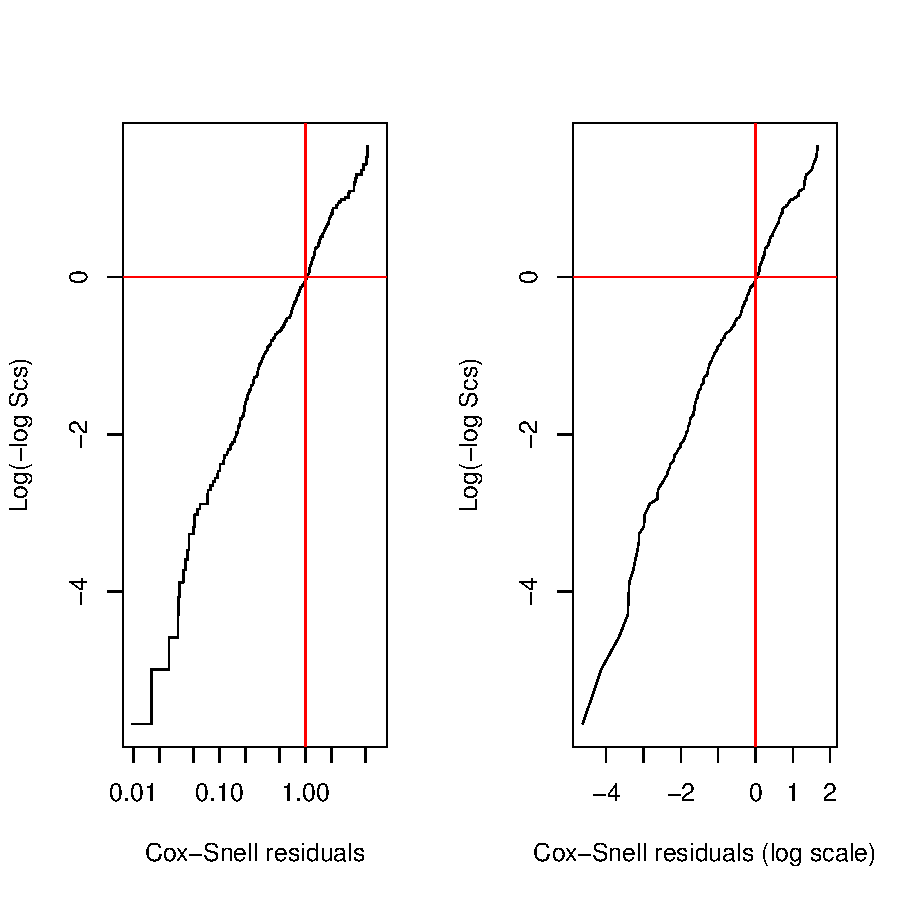
\includegraphics[width=3.5in]{coxsnell.pdf}}
{\bf Notes:}\\[2ex]
The fit from the Cox-Snell residuals is fairly good, which suggests that the model fits adequately.\\[2ex]
Nevertheless, Allison states that the ``Cox-Snell residuals...  are not very informative
for Cox models estimated by partial likelihood.''
%%%%%%%%%%%%%%%%%%%%%%%%%%%%%%%%%%%%%%%%%%%%%%%%%%%%%%%%%%%%%%%%%%%%%%%%%%%%
\subsection{Martingale Residuals}
See Fleming and Harrington, p.164. Martingale residuals are defined for the $i$-th individual as:

\[ r_i = \delta_i - \hat{\Lambda}(T_i) \]
~\\
\underline{\bf Properties:}
\begin{itemize}
\item $r_i$'s have mean 0
\item range of $r_i$'s is between $-\infty$ and 1
\item approximately uncorrelated (in  samples)
\item {\bf Interpretation:} - the residual $r_i$ can be viewed
as the difference between the observed number of deaths (0 or 1)
for subject $i$ between time 0 and $T_i$, and the expected numbers
based on the fitted model.
\end{itemize}
\noindent
Martingale residuals are obtained through the {\tt residuals} command (using {\tt type="martingale"}).
\\[2ex]
Once the martingale residual is created, you can plot it versus the
predicted log HR (i.e., $\bfbeta \bfZ_i$), or any of the individual
covariates.
\begin{figure}[h]
\caption{Martingale residuals in the halibut data example}
\centerline{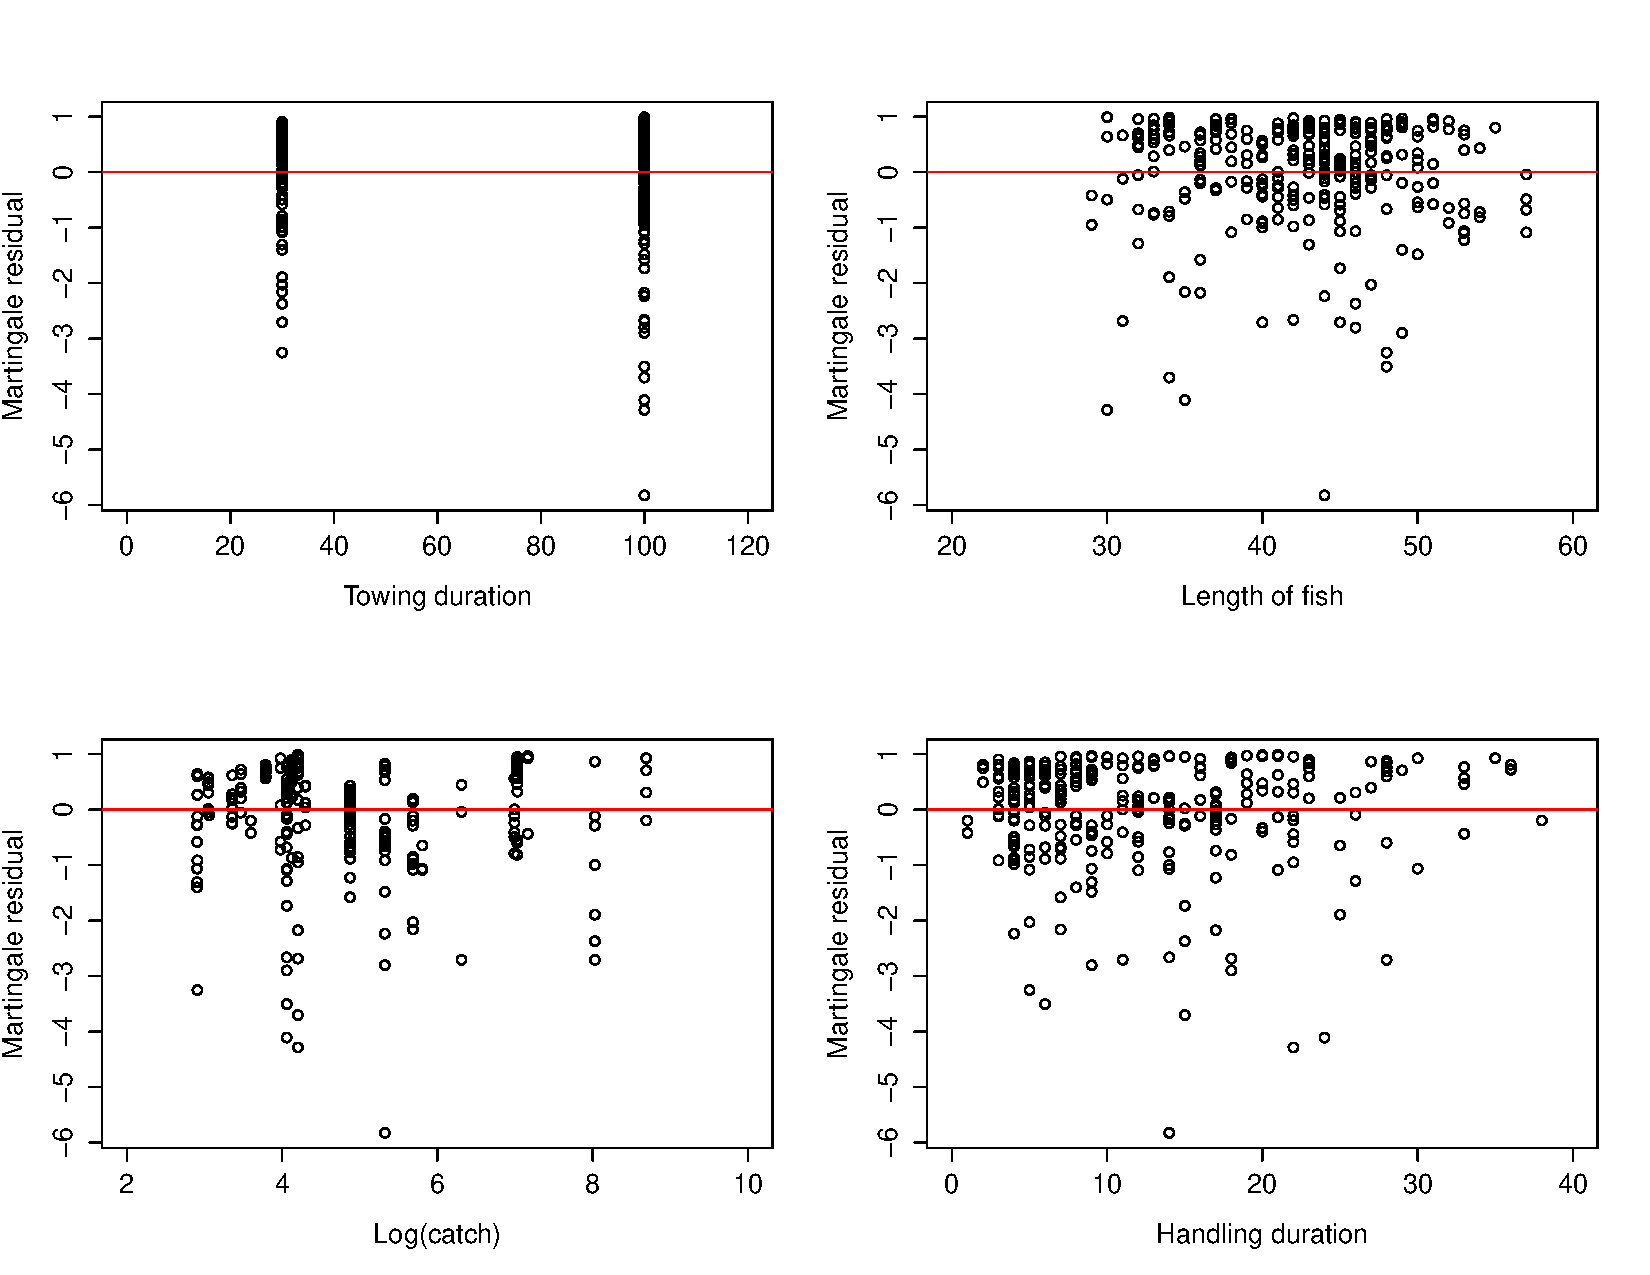
\includegraphics[width=3.5in]{mart_res.pdf}}
%%%%%%%%%%%%%%%%%%%%%%%%%%%%%%%%%%%%%%%%%%%%%%%%%%%%%%%%%%%%%%%%%%%%%%%%%%%%
\end{figure}
\begin{figure}[h]
\caption{Martingale residuals against the predicted log hazard ratio}
\centerline{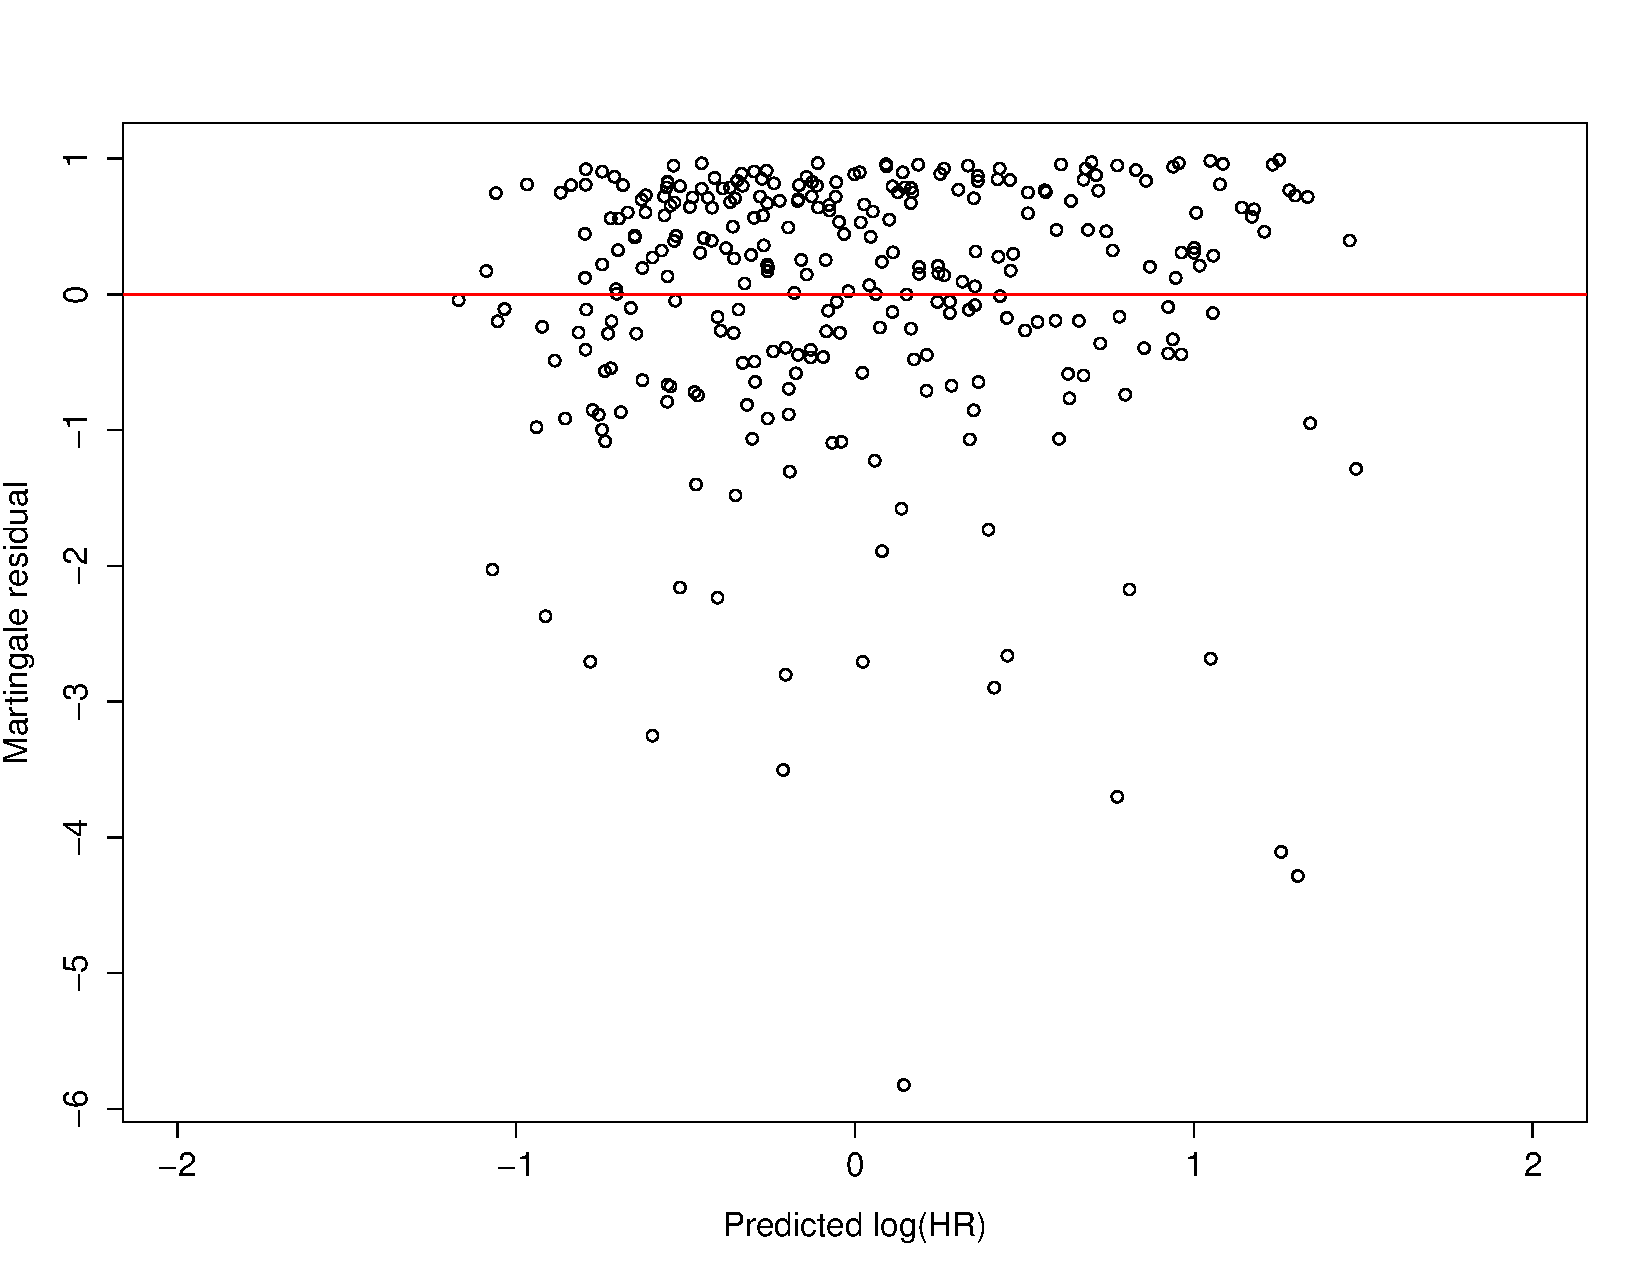
\includegraphics[width=3in]{martres_pred.pdf}}
\end{figure}
%%%%%%%%%%%%%%%%%%%%%%%%%%%%%%%%%%%%%%%%%%%%%%%%%%%%%%%%%%%%%%%%%%%%%%%%%%%%
\subsection{Deviance Residuals}
One problem with the martingale residuals is that they tend to be
asymmetric.
\\[2ex]
A solution is to use {\bf deviance residuals}.
For person $i$, these are defined as a function of the
martingale residuals ($r_i$):
\[ \hat{D}_i  =   \mbox{sign}(\hat{r}_i)  \sqrt{-2[\hat{r}_i +
                   \delta_i log(\delta_i-\hat{r}_i)]}  \]
{Obtaining deviance residuals in R}
In R, the deviance residuals are generated using {\tt residuals} command with the {\tt type="deviance"} option:
\noindent
The deviance residuals can then be plotted versus the predicted log(HR) or the
individual covariates, as shown for the Martingale residuals.
\\[2ex]
Deviance residuals behave much like residuals from OLS regression (i.e., mean=0, s.d.=1).  They are negative for observations with survival times that are smaller than expected.
%%%%%%%%%%%%%%%%%%%%%%%%%%%%%%%%%%%%%%%%%%%%%%%%%%%%%%%%%%%%%%%%%%%%%%%%%%%%
\begin{figure}[h!]
\caption{Deviance Residuals in the halibut data example}
\centerline{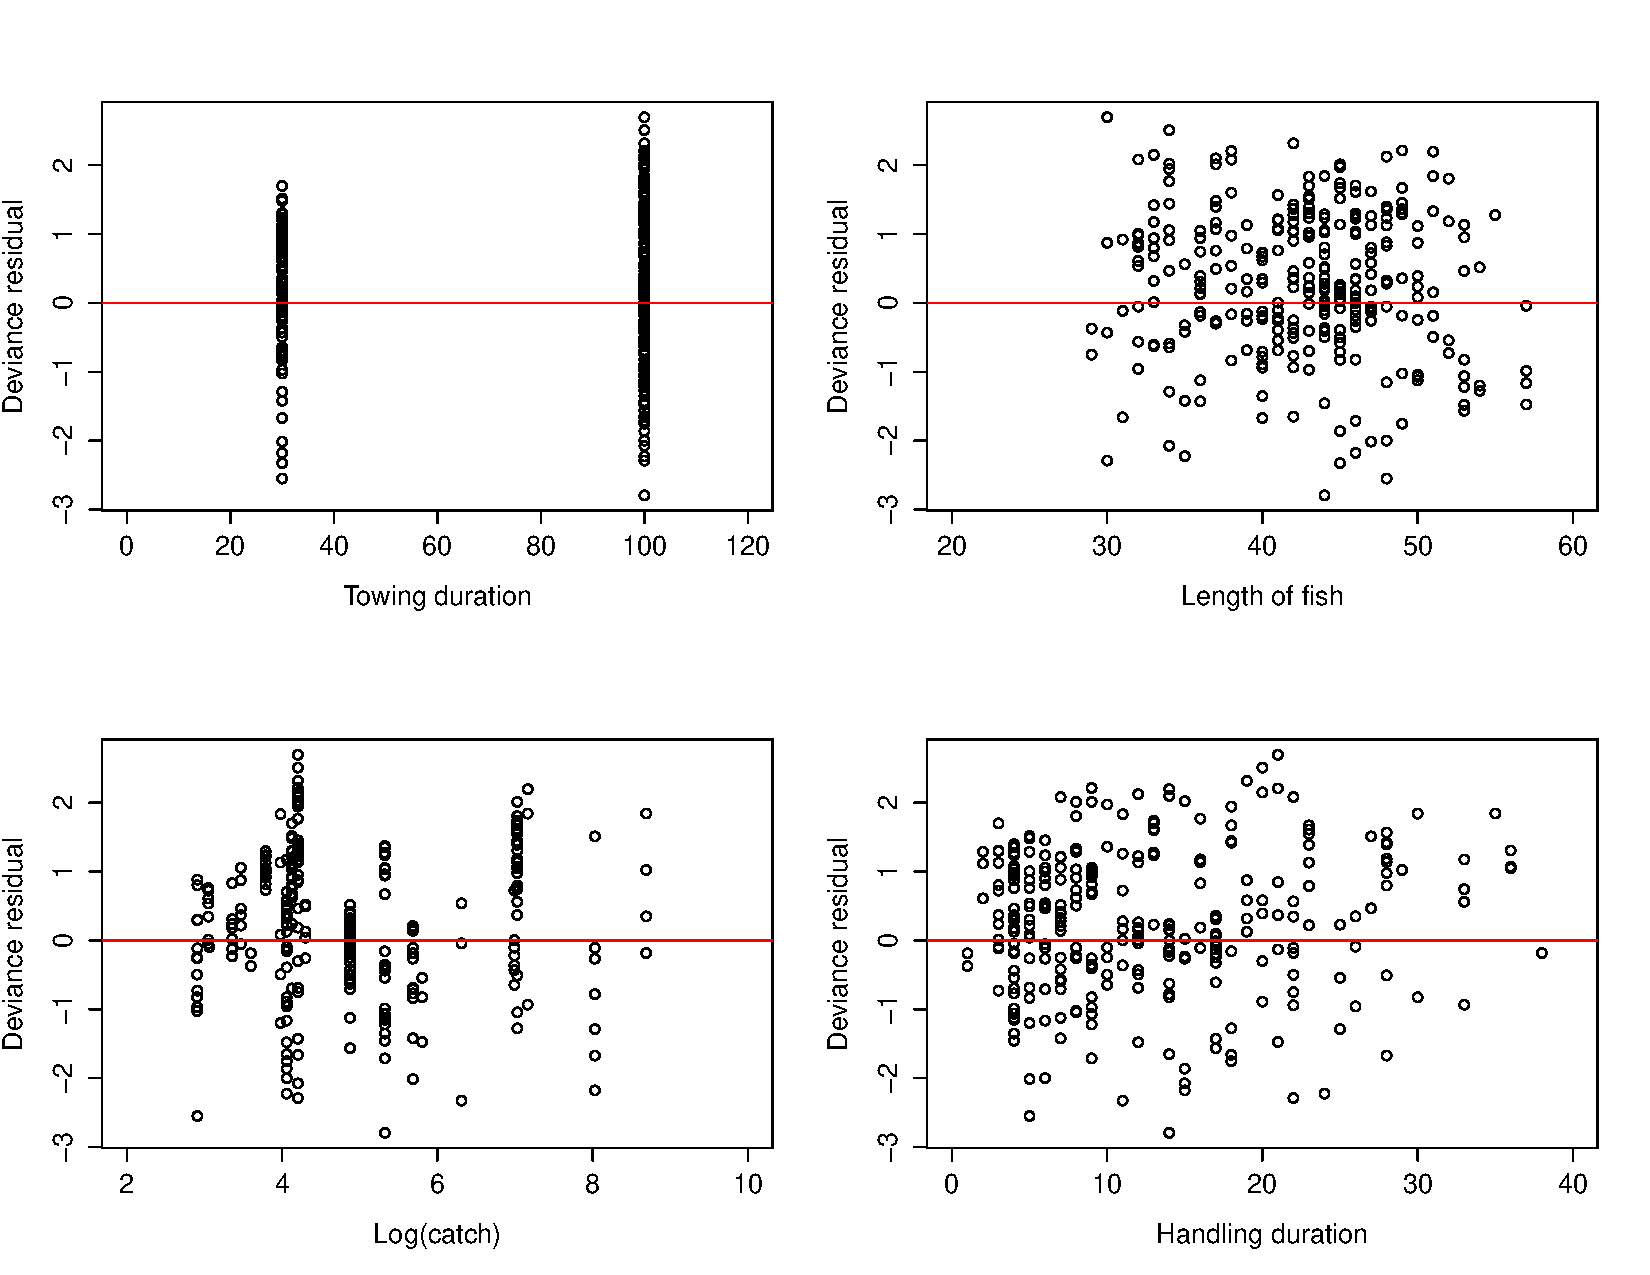
\includegraphics[width=4in]{dev_res.pdf}}
\end{figure}
\begin{figure}[h]
\caption{Deviance residuals versus predicted log hazard ratio}
\centerline{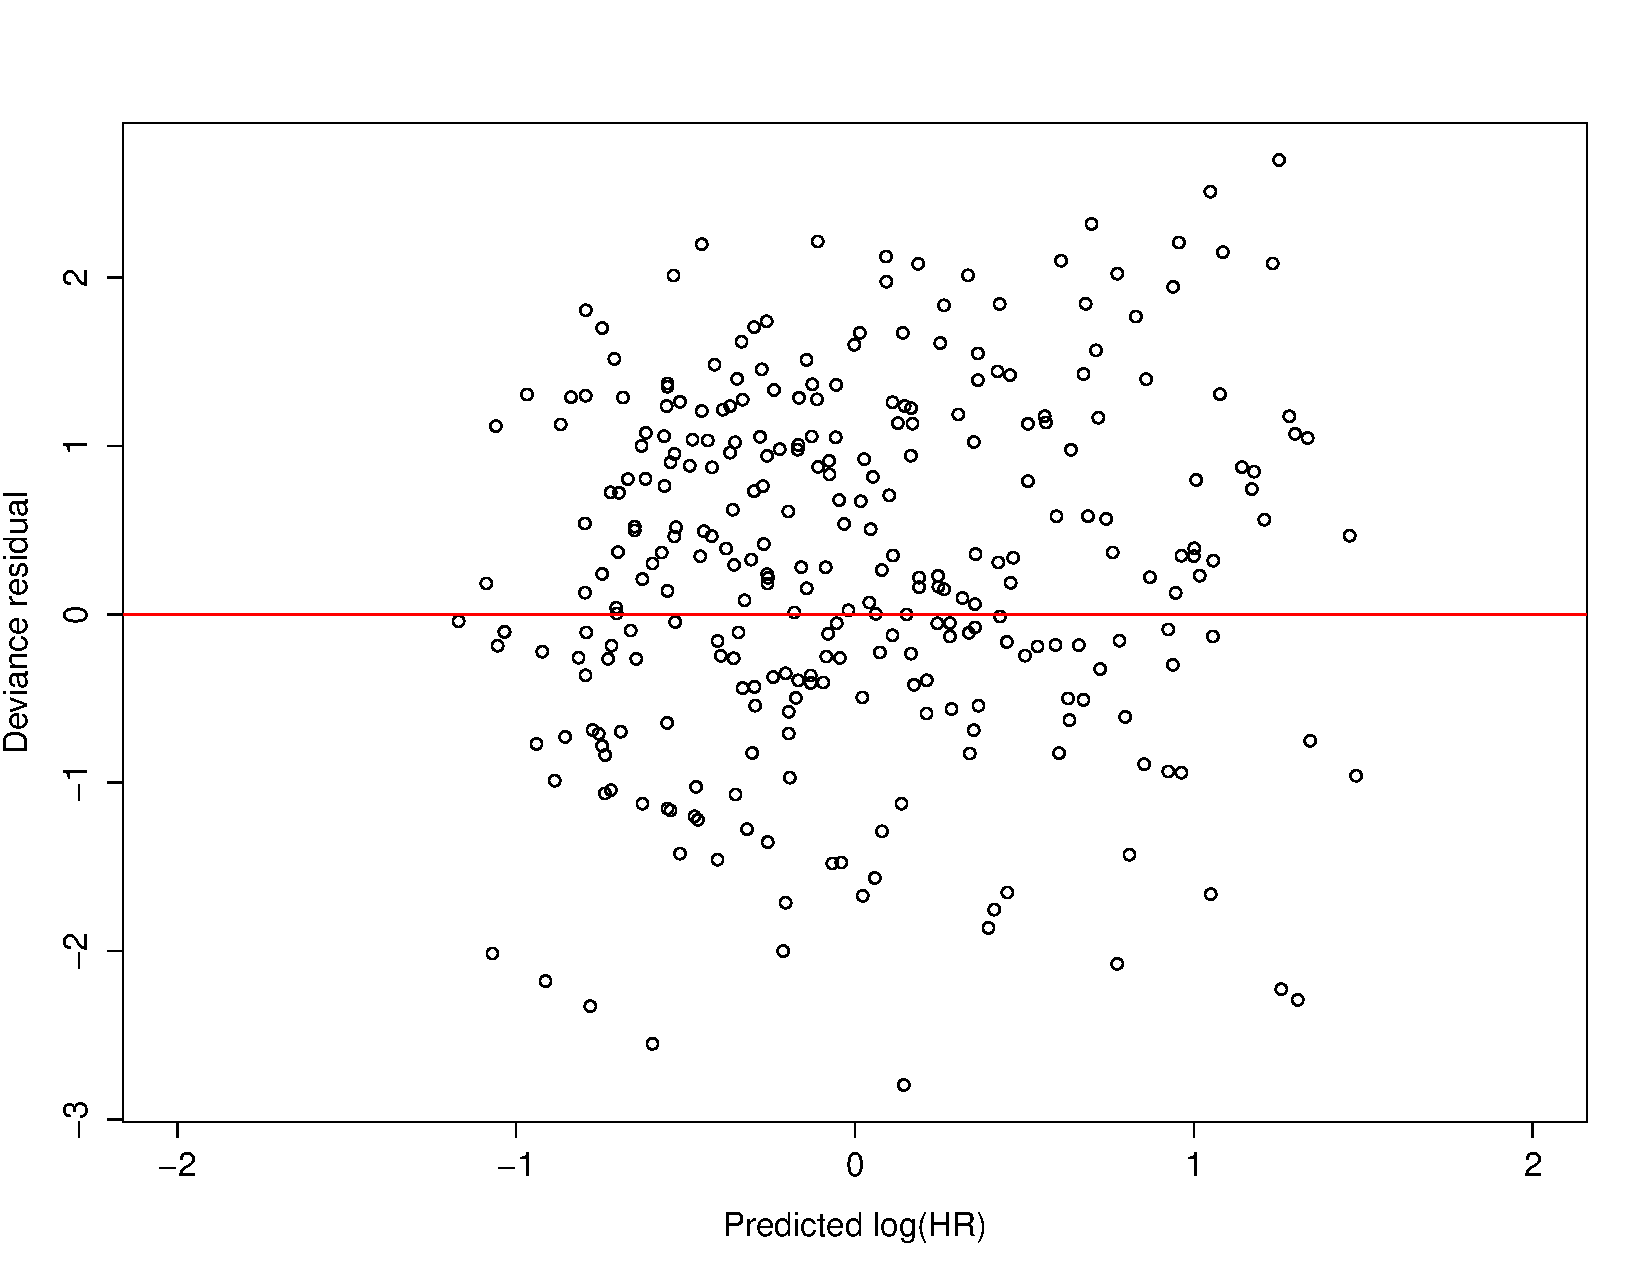
\includegraphics[width=3in]{devres_pred.pdf}}
\end{figure}
\subsection{Schoenfeld Residuals}
These are defined at each observed failure time as:
\[r_{ij}^s=Z_{ij}(t_i)-\bar{Z}_j(t_i)\]
\underline{Notes:}
\begin{itemize}
\item represent the difference between the observed covariate
and the average over the risk set at that time
\item calculated for each covariate
\item not defined for censored
failure times.
\item useful for assessing time trend or lack or proportionality,
based on plotting versus event time
\item sum to zero, have expected value zero, and
are uncorrelated (in  samples)
\end{itemize}
%%%%%%%%%%%%%%%%%%%%%%%%%%%%%%%%%%%%%%%%%%%%%%%%%%%%%%%%%%%%%%%%%%%%%%%%%%%%
In R, the Schoenfeld residuals are generated in the {\tt residuals}
command itself, using the {\tt type="schoenfeld"} option.

\begin{figure}[h!]
\caption{Schoenfeld residuals in the halibut data example}
\centerline{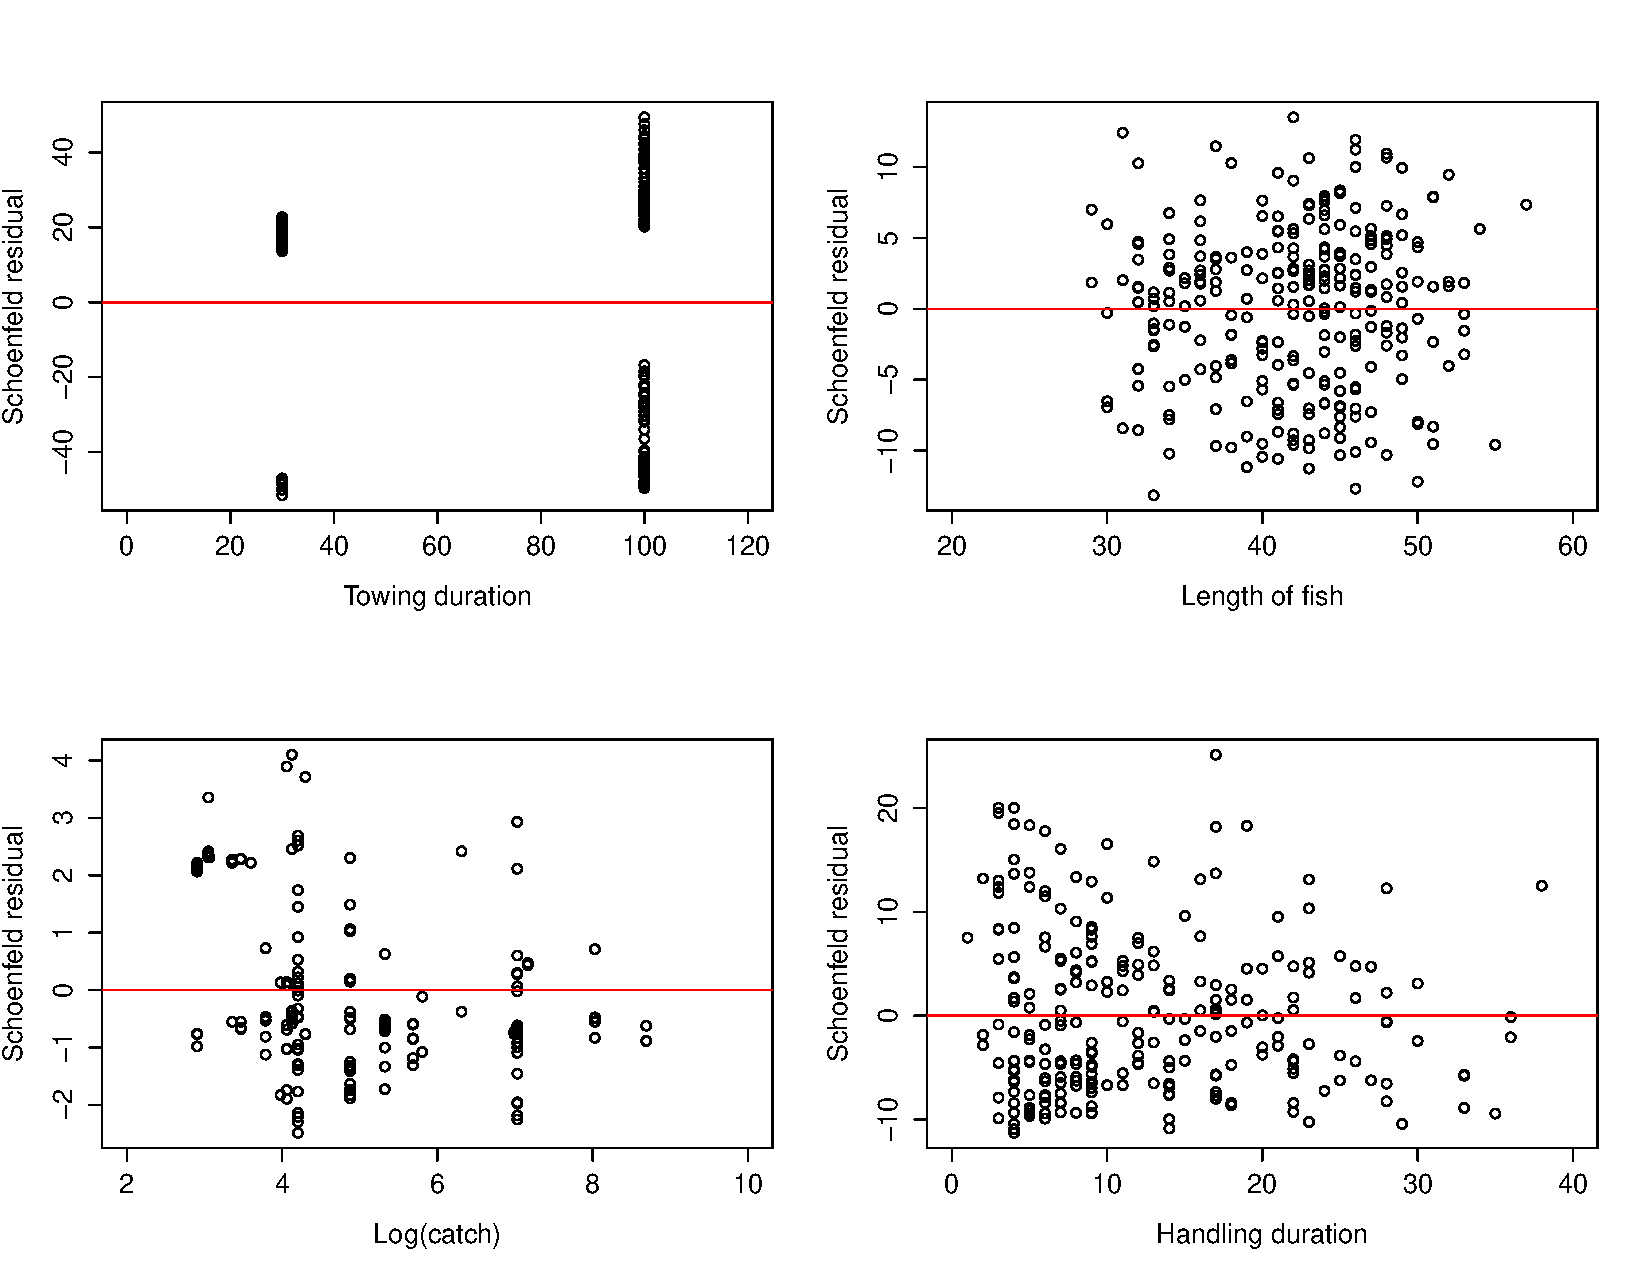
\includegraphics[width=4in]{sch_res.pdf}}
\end{figure}
\subsection{Weighted Schoenfeld residuals}
Weighted Schoenfeld Residuals are actually used more often than the previous unweighted
version, because they are more like the typical OLS residuals (i.e.,
symmetric around 0).
\\[2ex]
They are defined as:
\begin{eqnarray*}
r_{ij}^w & = & n \widehat{V}~ r_{ij}^s
\end{eqnarray*}

where $\widehat{V}$ is the estimated variance of $\hat{\bfbeta}$.  The weighted
residuals can be used in the same way as the unweighted ones to assess
time trends and lack of proportionality.
\\[2ex]
In R, use the command {\tt cox.zph} with the option.
\small
\begin{verbatim}
cox.zph(fit,transform = "identity")
\end{verbatim}
\normalsize
\newpage
This results in the following plots:
%\end{frame}
\begin{figure}[ht!]
\caption{Weighted Schoenfeld residuals}
\centerline{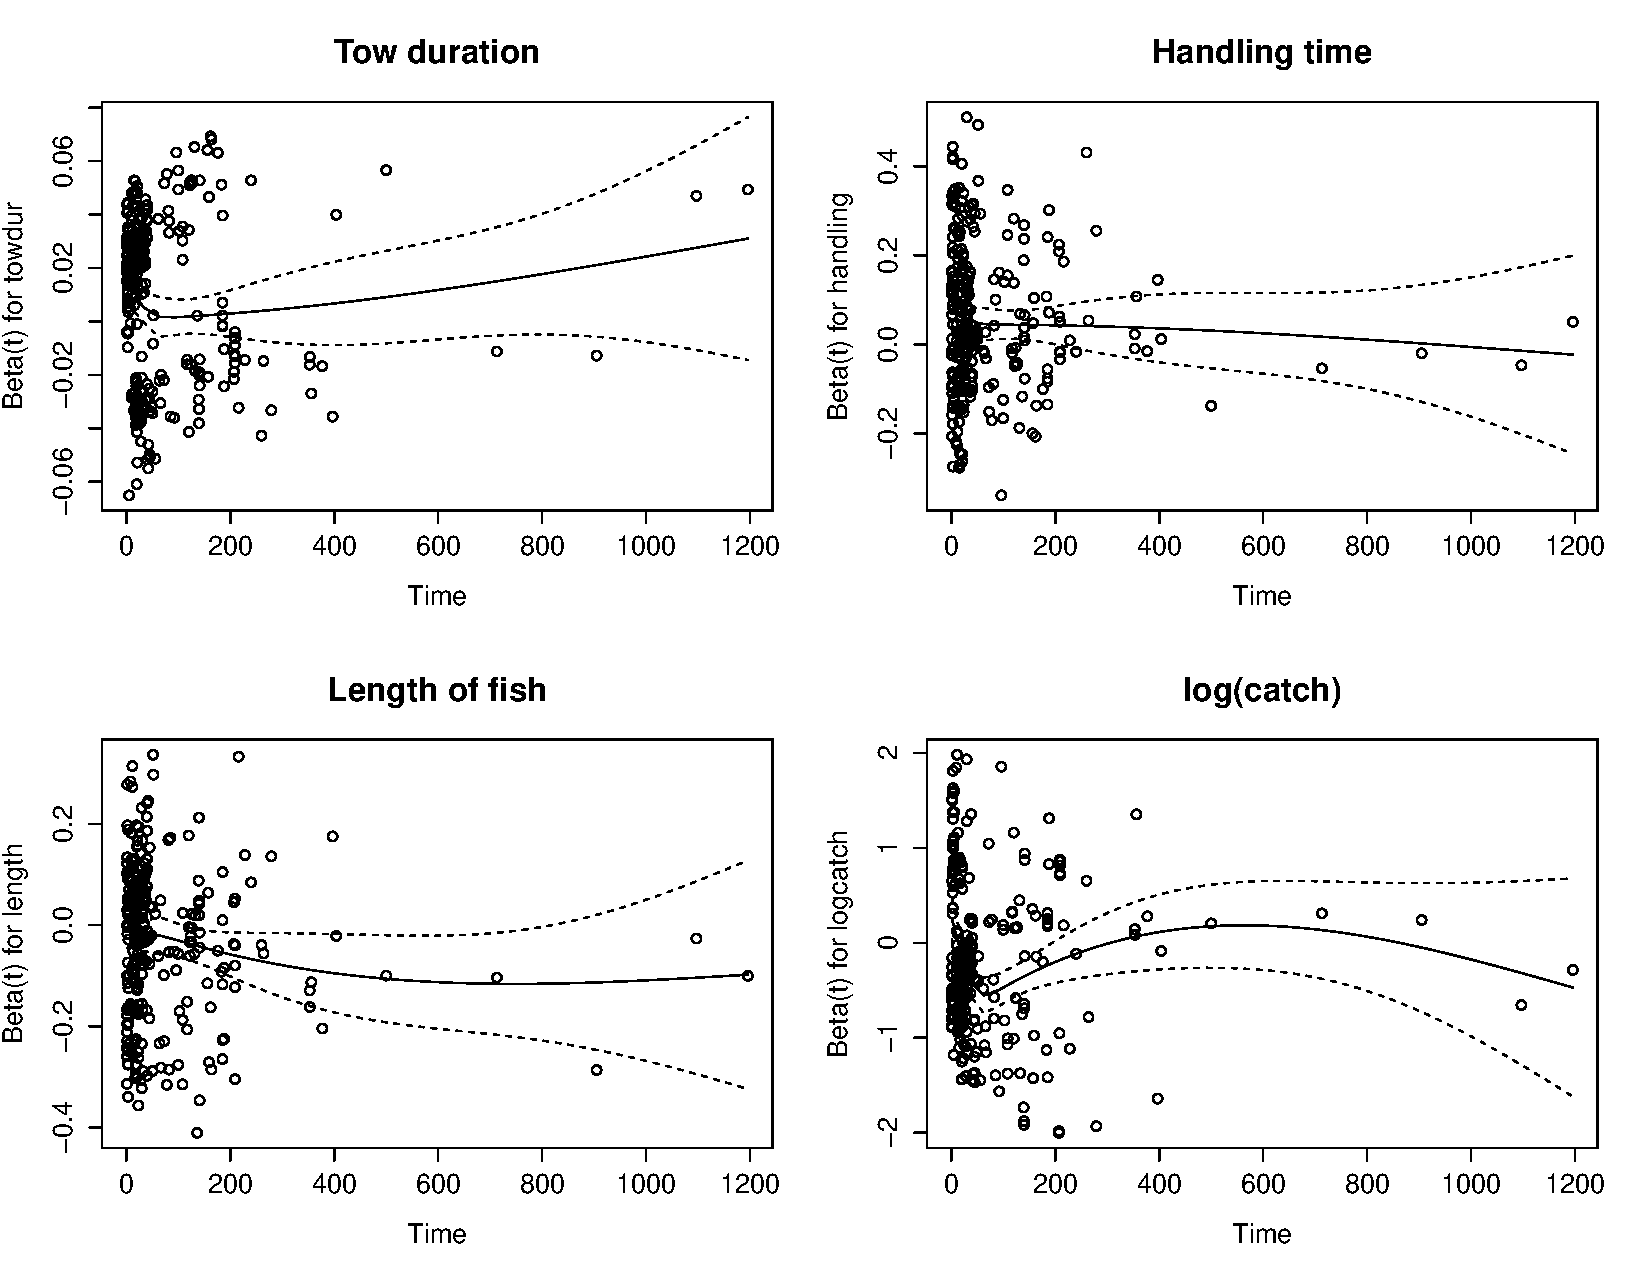
\includegraphics[width=4in]{wgt_sch_res.pdf}}
\end{figure}
\subsection{Using residual plots to identify relationships}
If you calculate martingale or deviance residuals
without any covariates in the model and then plot
against covariates, you obtain a graphical impression of the
relationship between the covariate and the hazard.
\\[2ex]
In R, it is easy to do this (also possible in stata using the
``estimate'' option)
\\[2ex]
We plot the martingale residuals versus each of the covariates. This produces the following plots:
\begin{figure}[ht!]
\caption{Residual plots}
\centerline{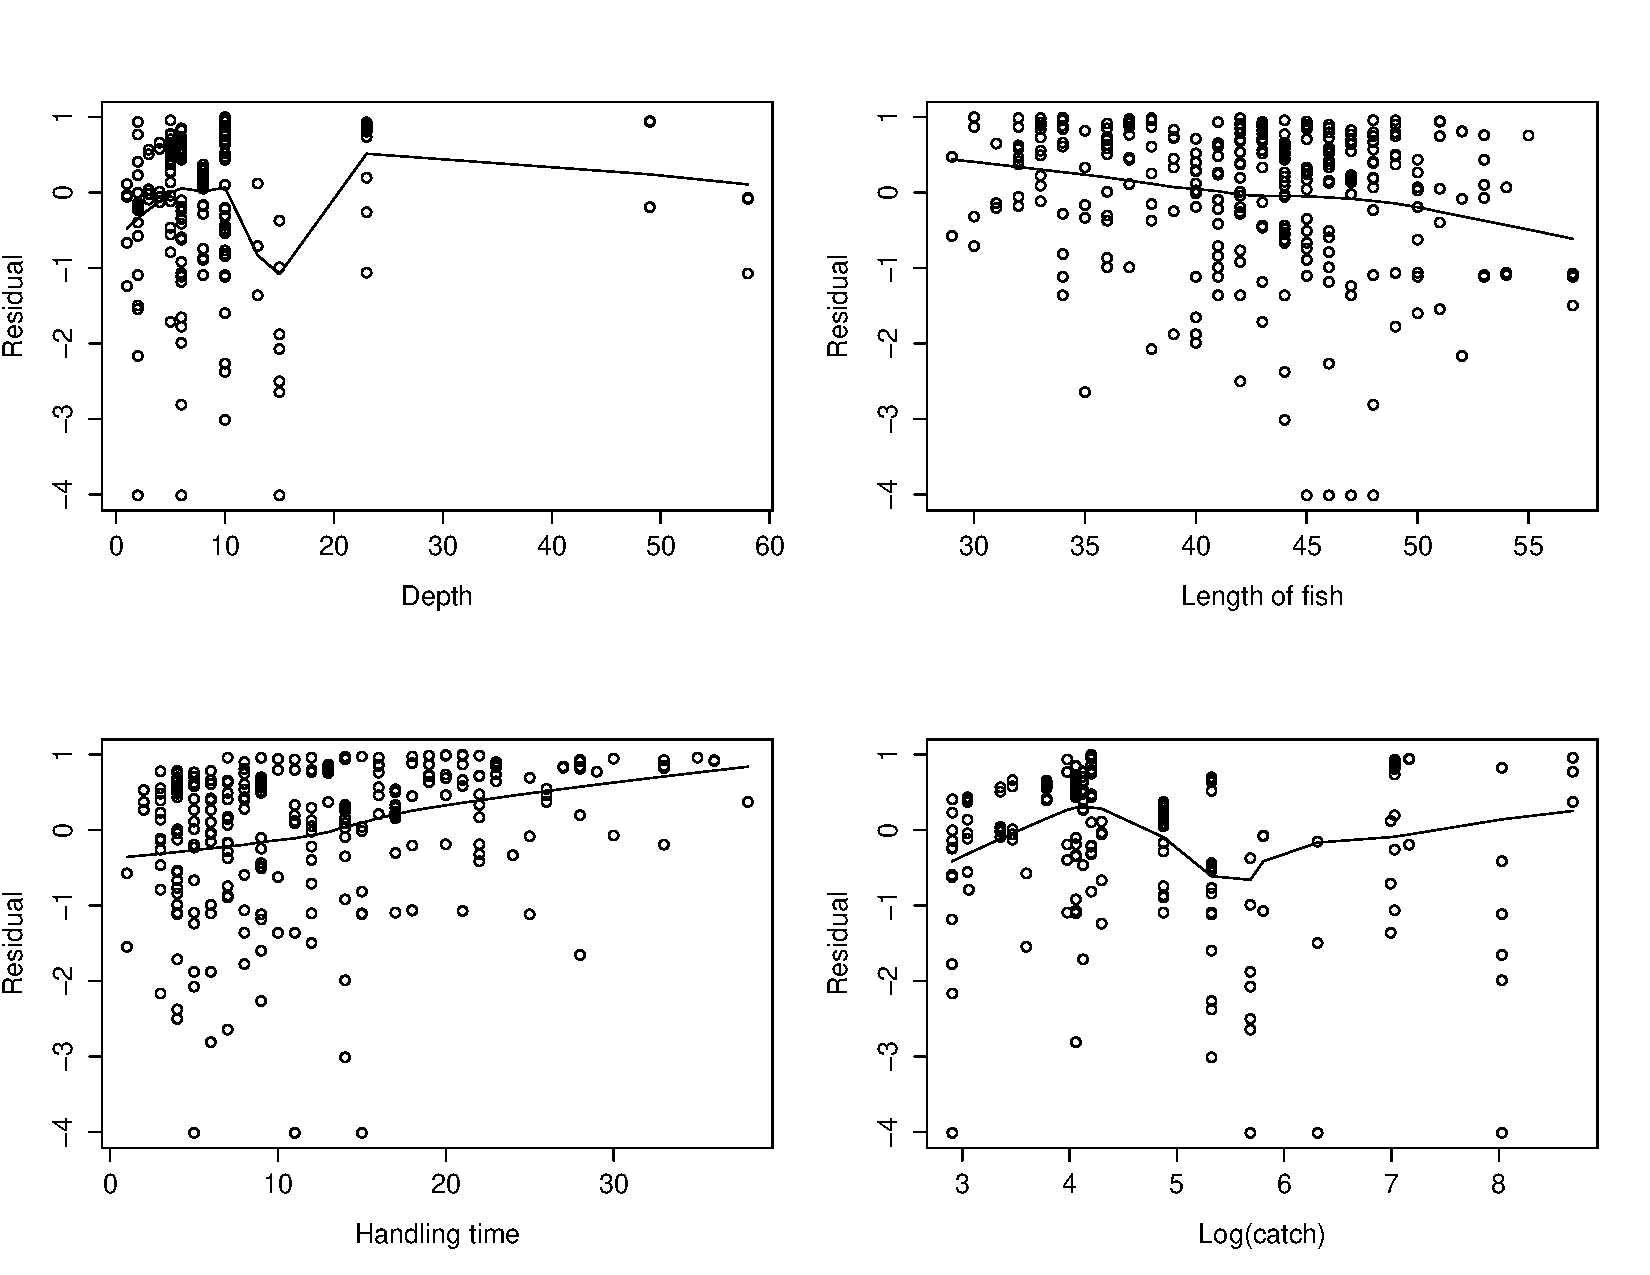
\includegraphics[width=3in]{res_plots.pdf}}
\end{figure}
%%%%%%%%%%%%%%%%%%%%%%%%%%%%%%%%%%%%%%%%%%%%%%%%%%%%%%%%%%%%%%%%%%%%%%%%%%%%
Can we improve the model?
\\[2ex]
The plots appear to have some structure, which indicate that
we could be leaving something out.  It is always a good idea
to check for interactions.
\\[2ex]
In this case, there are several important interactions.
I used a backward selection model forcing all main effects to be included,
and considering all pairwise interactions.
\newpage
\noindent
The results from this analysis are as follows:
\small
\begin{verbatim}
Call:
coxph(formula = Surv(survtime, censor) ~ towdur + depth + length +
    handling + logcatch + towdepth + lengthdepth + handlingdepth +
    towlength + towhandling, data = halibut)

  n= 294, number of events= 273

                    coef  exp(coef)   se(coef)      z Pr(>|z|)
towdur        -0.0756235  0.9271652  0.0174010 -4.346 1.39e-05 ***
depth          0.1249947  1.1331424  0.0639359  1.955 0.050583 .
length        -0.0775731  0.9253594  0.0255046 -3.042 0.002354 **
handling       0.0045787  1.0045892  0.0321858  0.142 0.886876
logcatch      -0.2241951  0.7991592  0.0715613 -3.133 0.001731 **
towdepth       0.0029236  1.0029279  0.0004994  5.854 4.79e-09 ***
lengthdepth   -0.0060456  0.9939727  0.0013568 -4.456 8.36e-06 ***
handlingdepth -0.0041262  0.9958823  0.0011834 -3.487 0.000489 ***
towlength      0.0011826  1.0011833  0.0003540  3.340 0.000836 ***
towhandling    0.0011146  1.0011152  0.0003556  3.134 0.001723 **
---
Signif. codes:  0 ‘***’ 0.001 ‘**’ 0.01 ‘*’ 0.05 ‘.’ 0.1 ‘ ’ 1

\end{verbatim}
\noindent
\normalsize
{\bf Interpretation:}
Handling alone doesn't seem to affect survival, unless it is combined
with a longer towing duration or shallower trawling depths.

\end{document} 